\chapter{Security Development Lifecycle}

Storicamente, la sicurezza del software veniva affrontata in modo reattivo: si 
sviluppava il codice e, solo alla fine, si facevano test di penetrazione o si 
aspettava che gli attaccanti trovassero le vulnerabilità per poi rilasciare una 
patch (approccio \textit{Penetrate and Patch}).

Questo approccio si è rivelato disastroso per diversi motivi ingegneristici ed 
economici:

\begin{itemize}
    \item \textbf{Ritardo nel rilevamento e risoluzione}: In media, ci vogliono 197 giorni 
    per rilevare una vulnerabilità e ulteriori 69 giorni per sviluppare e distribuire un fix.
    \item \textbf{Effetti collaterali delle patch}: Le patch sviluppate in fretta 
    introducono spesso nuove vulnerabilità o problemi di instabilità. Esempio di ciò 
    sono le prime patch rilasciate da Microsoft per mitigare la vulnerabilità 
    \textit{Meltdown}; a causa della fretta, la patch per Windows 7 ha introdotto 
    una vulnerabilità ben peggiore a livello software, permettendo a qualsiasi 
    processo in user-space di leggere e scrivere arbitrariamente in memoria.
    \item \textbf{Ritardo nell'applicazione dei fix}: Gli amministratori di sistema 
    sono spesso riluttanti ad applicare le patch per paura di causare disservizi 
    nei sistemi in produzione.
\end{itemize}

Per superare questo limite, nei primi anni 2000 inizia il primo approccio di uno 
sviluppo "sicuro" del software, l'iniziativa di Microsoft \textit{Trustworthy Computing Memo} 
è forse l'evento più significativo di questo cambiamento. L'industria ha iniziato ad 
integrare la sicurezza in ogni fase del ciclo di vita del software, portando alla 
formalizzazione del \textbf{Microsoft SDL} nel 2006.

\section{Microsoft SDL}

La fase di design è dove l'SDL garantisce il maggiore ritorno sull'investimento (ROI). 
Invece di scrivere codice e poi cercare i bug, si progetta un'architettura resiliente.

\begin{figure}[H]
    \centering
    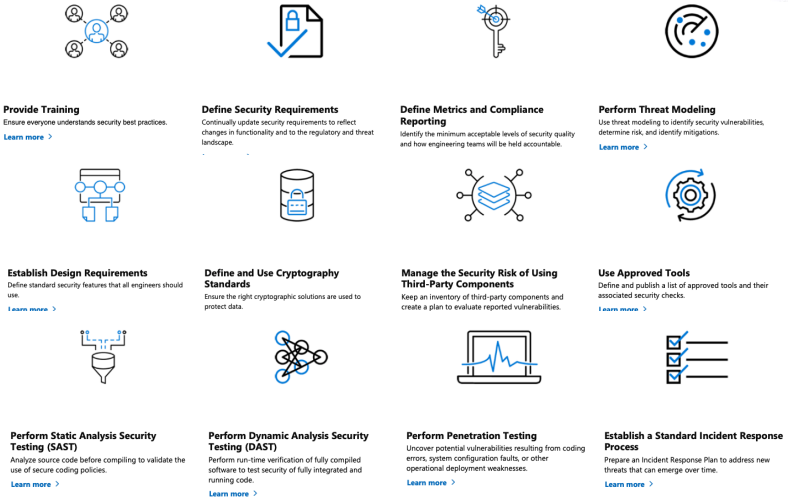
\includegraphics[width=1\linewidth]{img/capitolo8/sdl.png}
    \label{fig:sdl}
\end{figure}

\textbf{Provide Training}

Nella prima fase si sottolinea l'importanza di sensibilizzare i manager di un progetto, 
tutto il personale in generale, sulla Security. Coinvolgere tutti è importante e 
devono inoltre essere aggiornati sui principali strumenti e linguaggi volti alla sicurezza.

\textbf{Define Security Requirements}

In questa fase si raccolgono i requisiti si sicurezza fin dalle prime fasi dello sviluppo 
software. Fattori importanti da tenere in considerazione sono: requisiti di conformità
per la legalità e l'industria, standard interni ed esterni, informazioni raccolte dagli 
incidenti del passato e minacce note. 

Tecnica da utilizzare durante questa fase sono gli \textbf{Abuse Cases}: invece di 
limitarsi agli "Use Cases" (casi d'uso legittimi), si modellano gli Abuse Cases 
estendendo i diagrammi UML. Ad esempio in un'applicazione di e-commerce, mentre l'utente
legittimo ha gli use case "Login" e "Esegui un ordine", ci sono attori come il \textit{Cracker}
che cerca di "Rubare ID e password" (mitigato imponendo policy sulle password come il cambio 
periodico di esse) oppure l'\textit{Amministratore demotivato} che potrebbe "Manipolare la lista oggetti"
(mitigato da sistemi di validazione e log).

\textbf{Define Metrics and Compliance Reporting}

È legittimo avere un indicatore della Security del nostro prodotto; il problema è che non 
possiamo sapere e nemmeno misurare quante vulnerabilità ci siano nel nostro progetto software.
Per tale motivo le misure vengono condotte in modo indiretto: le metriche adottate prendono il 
nome di \textbf{KPIs}. Ci si chiede prima di tutto quanti difetti sulla sicurezza noti non sono stati 
ancora fixati e quanto tempo si è impiegato a risolverli. Le vulnerabilità critiche note 
devono essere fixate in una finestra temporale specifica.

\textbf{Perform Threat Modeling}

Il Threat Modeling serve a identificare falle di design prima di scrivere una singola 
riga di codice. Si utilizzano i \textbf{Data Flow Diagram (DFD)} per mappare i 
componenti del sistema (processi, datastore) e, soprattutto, i \textit{Trust Boundaries} tracciando ad esempio 
il confine tra una rete pubblica e un database interno.

Il Threat Modeling inoltre elenca le minacce in modo sistematico: per ogni componente 
si seleziona una o più minacce dalla tassonomia \textbf{STRIDE}:

\begin{itemize}
    \item \textbf{S}poofing (Falsificazione dell'identità)
    \item \textbf{T}ampering (Manomissione dei dati)
    \item \textbf{R}epudiation (Azioni non tracciabili/ripudiabili)
    \item \textbf{I}nformation Disclosure (Fuga di dati sensibili)
    \item \textbf{D}enial of Service (Compromissione della disponibilità)
    \item \textbf{E}levation of Privilege (Ottenere privilegi non autorizzati)
\end{itemize}

\begin{figure}[H]
    \centering
    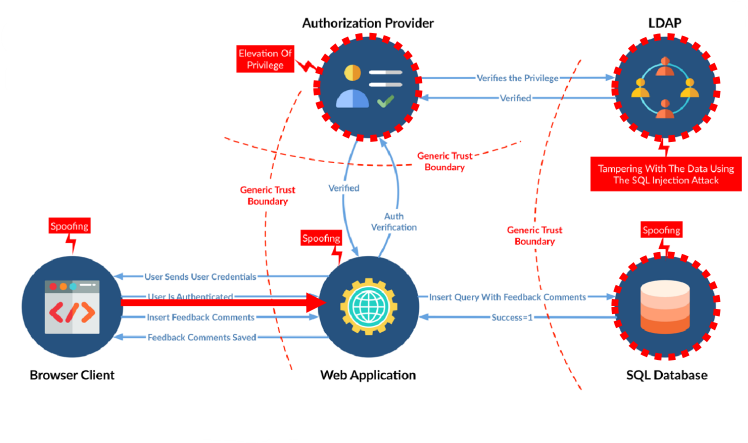
\includegraphics[width=1\linewidth]{img/capitolo8/stride.png}
    \label{fig:stride}
\end{figure}

L'esempio riportato in figura mostra l'interazione tra una Web Application e un Database SQL. 
Se un attaccante invia dati non validati, questa minaccia è classificata come \textit{Tampering} 
(tramite attacco \textit{SQL Injection}) perché altera i dati e il normale flusso di 
esecuzione della query sul DB.

\textbf{Establish Design Requirements}

Questi principi storici rimangono le fondamenta del \textit{secure design}; 
soffermiamoci su alcuni principi classici:

\begin{itemize}
    \item \textbf{Open Design}: Il design non deve basarsi sull'oscurità (\textit{security by obscurity}),
    infatti l'uso di credenziali hardcoded nel codice eseguibile è altamente sconsigliabile in quanto si 
    presume sempre che l'attaccante possa fare reverse engineering dell'eseguibile ed estrarre la stringa.
    \item \textbf{Least Privilege}: Un processo deve operare con i permessi minimi necessari. Esempio 
    di violazione di tale principio: un programma deve leggere un file di root all'avvio ma non esegue 
    un drop dei privilegi prima di chiamare un'altra applicazione, permettendo l'esecuzione di codice arbitrario 
    con privilegi massimi.
    \item \textbf{Fail-safe defaults}: All'occorrere di uno stato erroneo si deve procedere 
    ad eseguire un fall-back ad uno stato sicuro.
    \item \textbf{Economy of Mechanism}: Evitare complessità eccessiva (non necessaria) nei 
    meccanismi di sicurezza (es. REGEX DoS, IPSec).
\end{itemize}

\textbf{Define and Use Cryptography Standards}

Bisogna sempre utilizzare standard di crittografia chiari e riconosciuti dagli esperti, 
nonché di librerie di crittografia adeguatamente verificate. Microsoft stessa fornisce 
una pagina dedicata per assisterci sulla scelta dell'algoritmo di crittografia più 
giusto al caso nostro.

\textbf{Manage the Security Risk of Using Third-Party Components}

Il 95\% delle applicazioni moderne è composto da librerie open-source o di terze 
parti (con una media di 257 dipendenze per app). Non scriviamo la maggior parte del 
codice che eseguiamo, e questo apre scenari di attacco devastanti. Anche i componenti 
open source ritenuti sicuri possono avere vulnerabilità, bisogna quindi gestire in 
modo sicuro i vari componenti. Bisogna avere una mappa dei componenti che si sta 
utilizzando, dotarsi di un piano di risposta per analizzare, attraverso dei tool, la 
presenza o meno di possibili problemi. 

Inquinare un componente open source per arrivare ad attaccare un determinato prodotto 
software che fa uso di quel componente è un rischio concreto e ancora più grave della 
"semplice" vulnerabilità presente nel singolo componente. Sembra impensabile eppure è un 
rischio concreto: nel febbraio 2024 una backdoor malevola fu inserita all'interno di una 
libreria di OpenSSH.

\textbf{Use Approved Tools}

Anche gli strumenti di sviluppo devono essere approvati, meglio usare quelli originali.
È importante sottolinearlo siccome è successo nel passato che alcuni tool erano portatori
di malware come nel caso di \textit{XcodeGhost}: una versione pirata, ma anche malevola, 
del compilatore \textit{Xcode} per iOS.

\textbf{Perform Static/Dynamic Analysis Security Testing}

Una volta scritto il codice, vanno applicati tool di verifica automatici e manuali:

\begin{itemize}
    \item \textbf{SAST}: Analizzare il codice senza eseguirlo per trovare pattern di 
    codice insicuro, credenziali hardcoded, algoritmi crittografici deprecati, generatori 
    di numeri pseudocasuali deboli, ecc.
    \item \textbf{DAST}: Analizzare il programma in esecuzione inviando input malformati 
    per trovare vulnerabilità di sessione, difetti di autenticazione, dati sensibili 
    inviati in chiaro, ecc.
\end{itemize}

\textbf{Perform Penetration Testing}

Gli hacker \textit{white-hat} (etici) si fingono attaccanti e simulano azioni dannose 
sul sistema; si tratta quindi di un'attività che complementa l'attività di analisi statica/dinamica.

\textbf{Establish a Standard Incident Response Process}

Le organizzazioni devono essere preparate ad affrontare le inevitabili vulnerabilità.
Bisogna predisporre in modo proattivo un piano di risposta agli incidenti per stabilire:

\begin{itemize}
    \item chi contattare in caso di emergenza di sicurezza
    \item il protocollo per una mitigazione efficiente delle vulnerabilità
    \item il protocollo per la risposta ai clienti e la comunicazione
    \item il protocollo per la rapida implementazione di una correzione
\end{itemize}

\section{Agile}

Le metodologie Agile si basano su cicli iterativi molto brevi (gli \textit{Sprint}, che 
durano da 2-4 settimane, o anche rilasci giornalieri) e si concentrano soprattutto sui 
requisiti.

\begin{figure}[H]
    \centering
    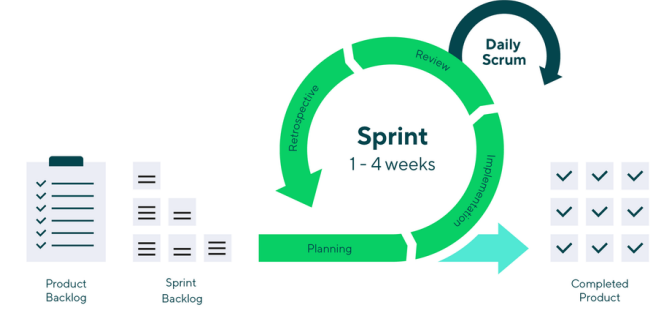
\includegraphics[width=1\linewidth]{img/capitolo8/agile.png}
    \label{fig:agile}
\end{figure}

Questo approccio entra in conflitto con il modello tradizionale del Security 
Development Lifecycle di Microsoft. L'SDL classico, infatti, prevede centinaia di 
requisiti obbligatori ed è pensato per prodotti con cicli di sviluppo lunghi, spesso 
di diversi anni. Negli ambienti Agile è necessario trovare un compromesso tra i 
requisiti di sicurezza e i tempi stretti di rilascio.

Per risolvere questo problema, l'\textbf{Agile SDL} organizza i requisiti di sicurezza in tre 
categorie:

\begin{itemize}
    \item \textbf{Every-Sprint requirements (Requisiti per ogni sprint)}: Sono attività fondamentali da fare 
    sempre per prevenire vulnerabilità critiche. Ad esempio bisognerebbe fare sempre il 
    \textit{Threat Modeling} per ogni nuova funzionalità introdotta o seguire le linee 
    guida per la validazione degli input.
    \item \textbf{One-time requirements (Requisiti una tantum)}: Attività da completare una sola volta 
    all'inizio del progetto o entro un periodo di grazia. Ad esempio configurare il 
    sistema di bug tracking o definire il \textit{Threat Model} di base dell'applicazione.
    \item \textbf{Bucket requirements (Requisiti a rotazione)}: Attività raggruppate in "secchi"; il team 
    deve pescare e completare un'attività da questi secchi periodicamente, spalmando 
    il carico di lavoro nel tempo. Ad esempio fare il \textit{fuzz testing} o revisionare il 
    design crittografico.
\end{itemize}

Il consorzio \textbf{SAFECode} fornisce linee guida specifiche per adattare la 
sicurezza ad Agile. Invece di imporre regole astratte, traduce le vulnerabilità 
(\textit{OWASP Top 10}) in:

\begin{itemize}
    \item \textbf{Security-focused stories}: Requisiti di sicurezza scritti come 
    \textit{User Stories}, ad esempio: "\textit{Come sviluppatore, voglio assicurarmi 
    che tutte le eccezioni siano gestite correttamente per evitare la perdita di dati 
    sensibili (CWE-754)}".
    \item \textbf{Operational security tasks}: Compiti operativi continui, come 
    tracciare le patch delle dipendenze di terze parti o utilizzare sempre le versioni 
    più recenti dei compilatori.
\end{itemize}

\section{Da DevOps a DevSecOps}

Il \textbf{DevOps} integra strettamente lo sviluppo (\textit{Dev}) e le operazioni di 
sistema (\textit{Ops}) per garantire consegne del software veloci e continue. Il 
\textbf{DevSecOps} fa un passo ulteriore: fonde le attività di sicurezza (\textit{Sec}) 
all'interno di tutto il ciclo DevOps, rendendola una responsabilità condivisa e 
continua.

L'implementazione del DevSecOps si basa su principi chiave:

\begin{itemize}
    \item \textbf{Uso di strumenti e Automazione}: I controlli di sicurezza devono 
    essere integrati nella pipeline CI/CD (\textit{Continuous Integration/Continuous 
    Deployment}). Questi strumenti devono generare pochi "falsi positivi" e non 
    devono richiedere agli sviluppatori competenze di sicurezza estreme.
    \item \textbf{Protezione delle Credenziali}: Nelle pipeline automatizzate c'è il 
    rischio di esporre dati sensibili (es. stringhe di connessione a database, chiavi 
    private, password hardcoded).
    \item \textbf{Apprendimento e Monitoraggio Continuo}: Monitorare le performance e 
    la sicurezza a \textit{run-time} per ridurre drasticamente i tempi necessari a 
    identificare e contenere un attacco.
\end{itemize}

\textbf{GitHub} è l'esempio più lampante dell'applicazione del DevSecOps e, in particolare, del 
concetto dello "\textit{Shift Left}", ovvero spostare i controlli di sicurezza il prima 
possibile nel ciclo di vita del software (verso sinistra in una classica linea 
temporale di sviluppo).

Invece di fare un \textit{Penetration Test} solo alla fine, con il rischio di dover 
riscrivere l'app intera se si trovano falle di design, si integrano analisi in ogni 
fase:

\begin{itemize}
    \item \textbf{Durante la scrittura del codice}: Plugin nell'IDE dello sviluppatore 
    e strumenti SAST analizzano il codice in tempo reale o durante la \textit{Pull Request}.
    \item \textbf{Durante la CI/Testing}: Vengono eseguiti controlli DAST sulle \textit{build}
    automatiche.
    \item \textbf{Fase finale}: I test di penetrazione e i programmi di \textit{Bug Bounty} 
    fungono da ultimo livello di garanzia.
\end{itemize}

\subsection{Maturità del DevSecOps}

L'ultimo concetto da affrontare è realistico: un'azienda che approccia la sicurezza 
per la prima volta non può essere sicura al 100\% dal giorno 1.

Per valutare a che punto si trova un'organizzazione, si usano i \textbf{Modelli di Maturità} come 
SAMM, BSIMM o l'OWASP DSOMM (\textit{DevSecOps Maturity Model}). 
Questi modelli classificano l'azienda su 5 livelli, dall'iniziazione fino all'ottimizzazione 
avanzata.

\begin{figure}[H]
    \centering
    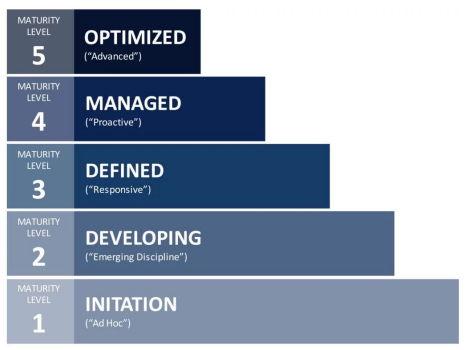
\includegraphics[width=0.6\linewidth]{img/capitolo8/devsecops.png}
    \label{fig:devsecops}
\end{figure}

Inizialmente, l'azienda implementerà strumenti base (SAST, DAST, SCA) con configurazioni 
standard, magari facendoli girare solo una volta a settimana o al mese. Le prime 
scansioni troveranno moltissimi errori, inclusi molti falsi positivi e gli sviluppatori 
potrebbero provare diffidenza verso questi nuovi strumenti che rallentano il loro 
lavoro. Le soluzioni proposte sono:

\begin{enumerate}
    \item \textbf{Iniziare a piccoli passi}: Non pretendere di risolvere tutto subito.
    \item \textbf{Non far fallire le build}: Nelle fasi iniziali, se uno strumento di 
    sicurezza rileva un problema, è meglio segnalarlo senza bloccare la compilazione 
    del software, per non fermare bruscamente la produzione.
    \item \textbf{Feedback immediato}: Fornire riscontri veloci agli sviluppatori 
    affinché possano correggere i problemi man mano che codificano.
\end{enumerate}